\chapter{Oxidación y reducción en química orgánica}\label{ch:b1:organic-redox}

Una botella de vino que se deja abierta se convierte en pocos días en
vinagre: unas bacterias usan el oxígeno del aire para oxidar el etanol a
ácido etanoico. Una cetona y el alcohol del que procede difieren en dos
átomos de hidrógeno y, si se cuenta bien, en dos electrones. Las
oxidaciones y reducciones orgánicas no se parecen a los intercambios de
electrones entre iones metálicos del \cref{ch:b1:nernst}, porque los
electrones viajan con protones o con iones hidruro, pero la contabilidad
es la misma. Este capítulo asigna \omterm{def:b1:organic-redox:oxidation-level}{niveles de oxidación} al carbono, los
usa para predecir qué da cada alcohol al oxidarse, y presenta los
reactivos hidruro que reducen los compuestos carbonílicos, atento a qué
grupos deja intactos cada reactivo.

\begin{recall}
Los \omterm{def:b1:nernst:oxidation-number}{números de oxidación}, las \omterm{def:b1:nernst:couple}{semiecuaciones} y el ajuste de las
ecuaciones redox están en el \cref{ch:b1:nernst}; las clases de alcoholes
y de carbonos, en el \cref{ch:b1:electronic-effects}; los \omterm{def:b1:acetals-protection:hemiacetal}{acetales} y la
\omterm{def:b1:acetals-protection:protecting-group}{protección} de los grupos carbonilo, en el \cref{ch:b1:acetals-protection};
las adiciones de Grignard, en el
\cref{ch:b1:organomagnesium}.
\end{recall}

\begin{omfigure}
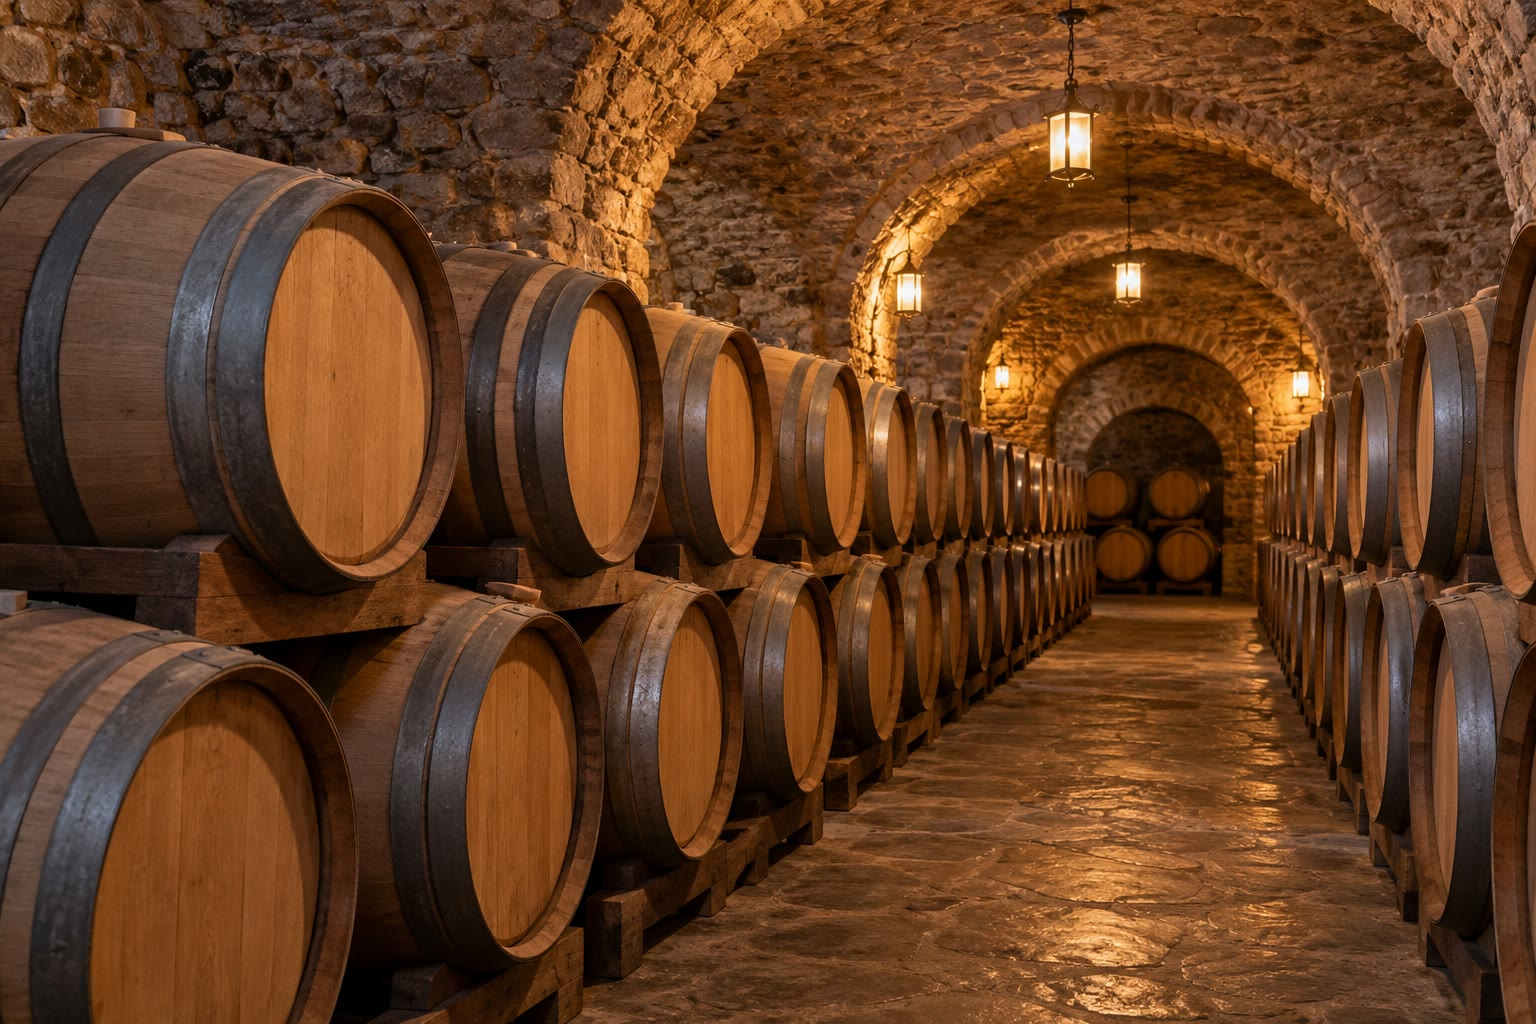
\includegraphics[width=0.58\linewidth]{images/book2/ai/b1-24-wine-cellar.jpg}

{\small Vino envejeciendo en una bodega. Protegido del aire, el vino
conserva su etanol; expuesto al aire, las bacterias acéticas lo oxidan a
ácido etanoico.}
\end{omfigure}

\section{Niveles de oxidación del carbono}

\begin{definition}[Nivel de oxidación]\label{def:b1:organic-redox:oxidation-level}
El \emph{nivel de oxidación}\index{nivel de oxidacion@nivel de oxidación} de un átomo de carbono es su
\omterm{def:b1:nernst:oxidation-number}{número de oxidación}, obtenido con las reglas de la
\cref{prop:b1:nernst:on-rules}: cada enlace con un átomo más
electronegativo (O, N, halógeno) cuenta $+1$, cada enlace con un
hidrógeno $-1$, cada enlace con otro carbono 0 (un enlace doble cuenta
dos veces).
\end{definition}

\begin{proposition}[Números de oxidación del carbono]\label{prop:b1:organic-redox:on-of-carbon}
El \omterm{def:b1:nernst:oxidation-number}{número de oxidación} de un carbono es igual al (número de enlaces con
O, N o halógenos) menos el (número de enlaces con H). Dentro de una misma
familia de compuestos con el mismo esqueleto carbonado, alcohol $\to$
aldehído o cetona $\to$ ácido carboxílico $\to$ dióxido de carbono es una
serie de oxidaciones de dos electrones cada una.
\end{proposition}

\begin{proof}
Rompiendo todos los enlaces y dando los dos electrones al compañero más
electronegativo: del H (menos electronegativo que el C), el carbono gana
un electrón, carga $-1$ por cada C--H; frente a O, N y halógenos (más
electronegativos) pierde uno, $+1$ por enlace; los enlaces C--C se
reparten a partes iguales. Al pasar de \ce{-CH2OH} ($-1$ para un carbono
unido a otro carbono) a \ce{-CHO} ($+1$) y a \ce{-COOH} ($+3$), el número
aumenta en 2 en cada etapa: dos electrones.
\end{proof}

\begin{omfigure}
\begin{tikzpicture}[font=\small, >={Stealth}]
  \foreach \x/\f/\n in {0/\ce{CH4}/-4, 2.4/\ce{CH3OH}/-2, 4.8/\ce{HCHO}/0, 7.2/\ce{HCOOH}/+2, 9.6/\ce{CO2}/+4} {
    \node[draw, rounded corners, minimum width=1.5cm] at (\x,0) {\f};
    \node[below] at (\x,-0.5) {$\n$};
  }
  \foreach \x in {0.8,3.2,5.6,8.0} \draw[->, thick, omThm] (\x,0) -- ++(0.8,0);
  \node[omThm, above] at (4.8,0.5) {oxidación: $-2\,\mathrm{e^-}$ (y $-2\,\ce{H+}$) en cada etapa};
  \node[left] at (-0.9,-0.75) {NO del C:};
\end{tikzpicture}

{\small Los \omterm{def:b1:organic-redox:oxidation-level}{niveles de oxidación} de la familia de un carbono: metano,
metanol, metanal, ácido metanoico, dióxido de carbono. Cada flecha es una
oxidación de dos electrones; leída al revés, una reducción.}
\end{omfigure}

\begin{method}[Ajustar una semiecuación orgánica]\label{met:b1:organic-redox:balance-organic-redox}
\begin{enumerate}
  \item Se escriben el \omterm{def:b1:nernst:couple}{oxidante} y el \omterm{def:b1:nernst:couple}{reductor} orgánicos con el mismo
        esqueleto.
  \item Se cuentan los electrones a partir del cambio de \omterm{def:b1:nernst:oxidation-number}{número de
        oxidación} de los carbonos que cambian (o, simplemente: dos por
        cada par de H perdido, o por cada O ganado).
  \item Se ajusta el oxígeno con agua, el hidrógeno con \ce{H+} y la carga
        con los electrones.
\end{enumerate}
Del etanol al ácido etanoico: \ce{CH3CH2OH + H2O -> CH3COOH + 4H+ + 4e-}.
Con dicromato acidificado (\ce{Cr2O7^2- + 14H+ + 6e- -> 2Cr^3+ + 7H2O}),
tres moléculas de etanol por cada dos iones dicromato:
\ce{3CH3CH2OH + 2Cr2O7^2- + 16H+ -> 3CH3COOH + 4Cr^3+ + 11H2O}.
\end{method}

\section{Oxidar los alcoholes}

\begin{proposition}[Qué dan los alcoholes al oxidarse]\label{prop:b1:organic-redox:alcohol-oxidation}
Un alcohol primario \ce{RCH2OH} se oxida al aldehído \ce{RCHO} y después
(en agua, con un \omterm{def:b1:nernst:couple}{oxidante} fuerte) al ácido carboxílico \ce{RCOOH}; un
alcohol secundario \ce{R2CHOH}, a la cetona \ce{R2CO}, que resiste una
oxidación posterior; un alcohol terciario \ce{R3COH} no se oxida sin
romper un enlace C--C.
\end{proposition}

\begin{proof}
La oxidación del alcohol elimina el hidrógeno del OH y un hidrógeno del
carbono carbinólico, formando el C=O. Un carbono carbinólico terciario no
tiene ese hidrógeno. El aldehído todavía lleva un H en el carbono
carbonílico; en agua está parcialmente hidratado, \ce{RCH(OH)2}, que se
oxida de nuevo del mismo modo a \ce{RCOOH}. Una cetona no tiene H en ese
carbono y se detiene.
\end{proof}

Los \omterm{def:b1:nernst:couple}{oxidantes} fuertes en agua --- el dicromato o el permanganato de
potasio acidificados --- oxidan los alcoholes primarios a ácidos. Para
detenerse en el aldehído, este se destila a medida que se forma (los
aldehídos hierven a menor temperatura que los alcoholes de los que
proceden, pues no tienen \omterm{def:b1:intermolecular-forces-solvents:hbond}{enlaces de hidrógeno} O--H), o se usan reactivos
más suaves y anhidros, descritos en el volumen del segundo año.

\begin{safety}{\ghs[5mm]{GHS03}\,\ghs[5mm]{GHS05}\,\ghs[5mm]{GHS06}\,\ghs[5mm]{GHS07}\,\ghs[5mm]{GHS08}\,\ghs[5mm]{GHS09}}
El dicromato de potasio, el \omterm{def:b1:nernst:couple}{oxidante} naranja clásico de los alcoholes,
está clasificado entre las sustancias que pueden causar cáncer: solo se
manipula en pequeñas cantidades, con guantes y gafas, y sus residuos de
cromo se recogen por separado; siempre que es posible se prefiere un
\omterm{def:b1:nernst:couple}{oxidante} menos peligroso.
% ledger: ghs:K2Cr2O7
\end{safety}

\section{Reducir los compuestos carbonílicos con hidruros}

\begin{definition}[Dador de hidruro]\label{def:b1:organic-redox:hydride-donor}
Un \emph{dador de hidruro}\index{dador de hidruro} transfiere un átomo de
hidrógeno con su par de enlace, \ce{H-}, a un carbono \omterm{def:b1:electronic-effects:nucleophile}{electrófilo}. El
borohidruro de sodio \ce{NaBH4} y el hidruro de litio y aluminio
\ce{LiAlH4} son \emph{hidruros metálicos complejos}\index{hidruro metalico complejo@hidruro metálico complejo}: el hidruro
se cede desde el ion \ce{BH4-} o \ce{AlH4-}, no como ion libre.
\end{definition}

\begin{omfigure}
\setchemfig{atom sep=2.1em}
\schemestart
\chemfig{H_3B^{-}-[@{bh}]@{h}H}
\+
\chemfig{@{c}C(-[:150]R)(-[:210]R')=[@{co}]@{o}O}
\arrow{->}
\chemfig{C(-[:150]R)(-[:210]R')(-[2]H)-O^{-}}
\arrow{->[\ce{H2O}]}
\chemfig{C(-[:150]R)(-[:210]R')(-[2]H)-OH}
\schemestop
\chemmove{\draw[->, thick, shorten <=2pt, shorten >=3pt](bh) .. controls +(80:9mm) and +(180:7mm) .. (c);
          \draw[->, thick, shorten <=2pt, shorten >=2pt](co) .. controls +(90:6mm) and +(90:6mm) .. (o);}
\par\vspace{6pt}

{\small Reducción de una cetona por el borohidruro: un par B--H forma el
nuevo enlace C--H mientras el par $\pi$ del C=O pasa al oxígeno; el
\omterm{def:b1:alcohol-activation:alkoxide}{alcóxido} se protona por el disolvente (agua o un alcohol) o en el
tratamiento. Cada \ce{BH4-} puede ceder sucesivamente sus cuatro
hidrógenos.}
\end{omfigure}

\begin{proposition}[Alcance de los dos hidruros]\label{prop:b1:organic-redox:hydride-scope}
El borohidruro de sodio, usado en agua o en alcoholes, reduce los
aldehídos a alcoholes primarios y las cetonas a alcoholes secundarios, y
deja intactos los ésteres, los ácidos carboxílicos, las amidas y los
enlaces dobles C=C. El hidruro de litio y aluminio, usado en éter seco,
reduce además los ésteres y los ácidos carboxílicos a alcoholes
primarios, y reacciona violentamente con el agua.
\end{proposition}

\begin{proof}
El enlace Al--H está más polarizado que el enlace B--H (el aluminio es
menos electronegativo que el boro), de modo que \ce{AlH4-} es un \omterm{def:b1:organic-redox:hydride-donor}{dador de
hidruro} mucho más fuerte, capaz de atacar el carbonilo menos \omterm{def:b1:electronic-effects:nucleophile}{electrófilo}
de los ésteres y de los carboxilatos; esa misma reactividad le hace
reaccionar con cualquier hidrógeno ácido, incluida el agua. \ce{BH4-}
reacciona solo lentamente con el agua y los alcoholes, y ataca solo los
carbonilos más \omterm{def:b1:electronic-effects:nucleophile}{electrófilos}. Un enlace C=C aislado no es \omterm{def:b1:electronic-effects:nucleophile}{electrófilo} y no
lo reduce ninguno de los dos.
\end{proof}

\section{Selectividad}

\begin{definition}[Reacción quimioselectiva]\label{def:b1:organic-redox:chemoselective}
Una \emph{reacción quimioselectiva}\index{reaccion quimioselectiva@reacción quimioselectiva} actúa sobre
un grupo funcional de una molécula en presencia de otros que, con otro
reactivo, también podrían reaccionar.
\end{definition}

\begin{omfigure}
\begin{tabular}{lcc}
\hline
grupo & \ce{NaBH4} (disolvente alcohólico) & \ce{LiAlH4} (éter seco) \\
\hline
aldehído \ce{RCHO} & alcohol primario & alcohol primario \\
cetona \ce{R2CO} & alcohol secundario & alcohol secundario \\
éster \ce{RCOOR} & no reacciona & dos alcoholes \\
ácido carboxílico \ce{RCOOH} & no reacciona (sal) & alcohol primario \\
alqueno \ce{C=C} & no reacciona & no reacciona \\
\omterm{def:b1:acetals-protection:hemiacetal}{acetal} & no reacciona & no reacciona \\
\hline
\end{tabular}

\smallskip
{\small Lo que reducen los dos hidruros. El borohidruro de sodio es el
reactivo quimioselectivo; el hidruro de litio y aluminio, el potente.}
\end{omfigure}

\begin{example}[Un cetoéster]\label{ex:b1:organic-redox:ketoester}
El 4-oxopentanoato de etilo, \ce{CH3CO(CH2)2COOEt}, da con borohidruro de
sodio el 4-hidroxipentanoato de etilo: solo se reduce la cetona. Con
hidruro de litio y aluminio se reducen los dos grupos: pentano-1,4-diol
(y etanol). Para reducir solo el éster, antes hay que proteger la cetona
como \omterm{def:b1:acetals-protection:hemiacetal}{acetal} (\cref{ch:b1:acetals-protection}).
\end{example}

\begin{inthelab}[Reducir una cetona]
Se añade el borohidruro de sodio en pequeñas porciones a una disolución
fría de la cetona en etanol: la reacción es exotérmica, y burbujea
hidrógeno procedente de la reacción lenta del reactivo con el disolvente.
Tras agitar, un ácido diluido destruye el exceso de reactivo (más
hidrógeno: ninguna llama cerca) y se extrae el alcohol. El hidruro de
litio y aluminio, en cambio, solo se usa en éter seco bajo gas inerte, y
su exceso se destruye con gran cuidado.
\end{inthelab}

\section{Ejercicios}

\begin{exercise}[$\star$]\label{exo:b1:organic-redox:1}
Dese el \omterm{def:b1:nernst:oxidation-number}{número de oxidación} de cada carbono en el etanol, el etanal, el
ácido etanoico, la propanona y el ácido metanoico.
\end{exercise}

\begin{exercise}[$\star$]\label{exo:b1:organic-redox:2}
¿Qué da el dicromato acidificado con el propan-1-ol, el propan-2-ol y el
2-metilpropan-2-ol?
\end{exercise}

\begin{exercise}[$\star$]\label{exo:b1:organic-redox:3}
Escríbanse las \omterm{def:b1:nernst:couple}{semiecuaciones} de los pares propanona/propan-2-ol y
etanal/etanol en medio ácido.
\end{exercise}

\begin{exercise}[$\star$]\label{exo:b1:organic-redox:4}
¿Qué dan el borohidruro de sodio y el hidruro de litio y aluminio con el
butanal, la butanona, el butanoato de etilo y el ácido butanoico?
\end{exercise}

\begin{exercise}[$\star\star$]\label{exo:b1:organic-redox:5}
Ajústese la oxidación del propan-2-ol por el permanganato en medio ácido
(\ce{MnO4-}/\ce{Mn^2+}) y calcúlese el volumen de permanganato de
\qty{0.020}{mol/L} necesario para \qty{1.20}{g} de alcohol ($M = \qty{60.0}{g/mol}$).
\end{exercise}

\begin{exercise}[$\star\star$]\label{exo:b1:organic-redox:6}
¿Cómo puede obtenerse propanal a partir del propan-1-ol sin que se oxide
más? Úsense las temperaturas de ebullición: propan-1-ol
\qty{97}{\celsius}, propanal
\qty{48}{\celsius}.
% ledger: bp:propanal, bp:propan-1-ol
\end{exercise}

\begin{exercise}[$\star\star$]\label{exo:b1:organic-redox:7}
Escríbase el mecanismo de la reducción del etanal por \ce{BH4-} en
etanol. ¿Qué átomo del producto procede del reactivo?
\end{exercise}

\begin{exercise}[$\star\star$]\label{exo:b1:organic-redox:8}
La reducción de la butanona con \ce{NaBH4} da un alcohol \omterm{def:b1:stereochemistry-in-depth:stereocentre}{quiral}. ¿Es
ópticamente activo? ¿Por qué?
\end{exercise}

\begin{exercise}[$\star\star$]\label{exo:b1:organic-redox:9}
En la prueba de alcoholemia en aliento que usaba antes la policía, el
dicromato naranja se volvía verde. Escríbase la reacción con el etanol y
explíquese el cambio de color.
\end{exercise}

\begin{exercise}[$\star\star\star$]\label{exo:b1:organic-redox:10}
Propónganse síntesis de: el 2-metilbutan-2-ol a partir del etanal y de un
\omterm{def:b1:organomagnesium:organometallic}{reactivo de Grignard}, seguidos de una oxidación y de una segunda etapa de
Grignard; el pentan-3-ol a partir del propanal. Cuéntense las oxidaciones
y las reducciones.
\end{exercise}

\begin{exercise}[$\star\star\star$]\label{exo:b1:organic-redox:11}
Redúzcase solo el grupo éster del 4-oxopentanoato de metilo,
\ce{CH3CO(CH2)2COOCH3}. Planifíquense las tres etapas con una \omterm{def:b1:acetals-protection:protecting-group}{protección}
y dese el producto.
\end{exercise}

\begin{exercise}[$\star\star\star$]\label{exo:b1:organic-redox:12}
Demuéstrese que en la oxidación de un alcohol primario al ácido se
intercambian cuatro electrones, mediante los \omterm{def:b1:nernst:oxidation-number}{números de oxidación} y
mediante la \omterm{def:b1:nernst:couple}{semiecuación}. Generalícese a la oxidación del metano a
dióxido de carbono.
\end{exercise}

\section{Problema: del ciclohexanol al ácido adípico}

\begin{problem}[{Problema de fin de semana --- los niveles de oxidación en
el ciclohexanol, la ciclohexanona y el ácido adípico, la oxidación por el
ácido nítrico y sus electrones, una vía con peróxido de hidrógeno, y la
masa de óxido de dinitrógeno liberada por tonelada de ácido adípico}]
\label{pb:b1:organic-redox:1}
El ácido adípico, ácido hexanodioico \ce{HOOC(CH2)4COOH}, se fabrica a
gran escala para los nailones, sobre todo por oxidación del ciclohexanol
(con ciclohexanona) por el ácido nítrico, que libera óxido de dinitrógeno
\ce{N2O}, un potente gas de efecto invernadero. Masas molares
(\unit{g/mol}): \ce{C6H12O} 100.0,
\ce{C6H10O} 98.0, \ce{C6H10O4} 146.0, \ce{N2O} 44.0, \ce{HNO3} 63.0,
\ce{H2O2} 34.0.

\medskip
\noindent\textbf{Parte I --- \omterm{def:b1:organic-redox:oxidation-level}{Niveles de oxidación}.}
\begin{enumerate}
  \item Dese el \omterm{def:b1:nernst:oxidation-number}{número de oxidación} de cada carbono del ciclohexanol.
  \item Lo mismo para la ciclohexanona.
  \item Lo mismo para el ácido adípico.
  \item ¿Qué carbonos se oxidan al pasar del ciclohexanol al ácido
        adípico, y qué enlace se rompe?
  \item ¿Cuántos electrones pierde una molécula de ciclohexanol?
  \item ¿Por qué la ciclohexanona, una cetona, se oxida aquí sin embargo
        aún más?
\end{enumerate}

\medskip
\noindent\textbf{Parte II --- La vía del ácido nítrico.}
\begin{enumerate}[resume]
  \item Escríbase la \omterm{def:b1:nernst:couple}{semiecuación} del ciclohexanol al ácido adípico en
        medio ácido.
  \item Dese el \omterm{def:b1:nernst:oxidation-number}{número de oxidación} del N en \ce{HNO3} y en \ce{N2O}.
  \item Escríbase la \omterm{def:b1:nernst:couple}{semiecuación} \ce{HNO3}/\ce{N2O}.
  \item Combínense; compruébese que se obtiene
        \ce{C6H12O + 2HNO3 -> C6H10O4 + N2O + 2H2O}.
  \item ¿Cuántos moles de electrones se intercambian por mol de ácido
        adípico?
  \item Calcúlese la masa de ácido nítrico consumida por tonelada de ácido
        adípico.
\end{enumerate}

\medskip
\noindent\textbf{Parte III --- Una vía con peróxido de hidrógeno.}
\begin{enumerate}[resume]
  \item Escríbase la \omterm{def:b1:nernst:couple}{semiecuación} \ce{H2O2}/\ce{H2O}.
  \item Escríbase y ajústese la oxidación del ciclohexanol por el peróxido
        de hidrógeno a ácido adípico.
  \item Calcúlese la masa de \ce{H2O2} por tonelada de ácido adípico.
  \item ¿Cuál es el único subproducto? ¿Por qué se dice que esta vía es
        más verde?
  \item El peróxido de hidrógeno debe ser activado por un \omterm{def:b1:elementary-steps:catalyst}{catalizador}.
        Con ayuda del \cref{exo:b1:nernst:12}, explíquese por qué una
        oxidación termodinámicamente favorecida puede necesitar uno
        todavía.
  \item ¿Qué haría el borohidruro de sodio con la ciclohexanona?
        Escríbase la reacción.
\end{enumerate}

\medskip
\noindent\textbf{Parte IV --- Las masas y el gas de efecto invernadero.}
\begin{enumerate}[resume]
  \item Calcúlese la cantidad de ácido adípico en una tonelada.
  \item Calcúlese la cantidad de \ce{N2O} que se forma con ella por la vía
        nítrica.
  \item Calcúlese la masa de ciclohexanol necesaria por tonelada, con un
        \omterm{def:b1:extent-q-and-k:fractional-extent}{rendimiento} del \qty{95}{\percent}.
  \item Dese la masa de \ce{N2O} liberada por tonelada de ácido adípico
        por la vía nítrica, en toneladas.
\end{enumerate}
\end{problem}
